\chapter{Introduction}

\section{AI in games}

Artificial intelligence refers to techniques used in computer and video games to produce the illusion of intelligence in the behavior of non-player characters (NPCs). The techniques used typically draw upon existing methods from the field of artificial intelligence (AI).

Developing game AI, i.e. the algorithms that control NPCs in a game, is well-known to be a difficult problem. Three outstanding challenges contribute to this difficulty. 
First, game developers have little time allocated to develop game AI; other aspects of game development such as storyline, graphics, and network connections usually take precedence. Second, the development of environments, called level design, is typically done independently of the development of the game AI. Yet, game AI will be controlling NPCs running in these environments. Third, games change over time.
\footnote{During our work we faced all of these problems (even if we are not game developers!). We had little time to share with other homeworks/projects/exams, design was a ripoff of graphics from other games and our vision of the game kept changing during development process!!}

One of the most fundamental requirements (not the only one!!) of AI is to move characters around in the game sensibly. Even the earliest AI-controlled characters (the ghosts in Pac-Man or the opposing bat in some Pong variants) had movement algorithms that weren't far removed from the games of today.

Movement forms the lowest level of AI techniques. Many games rely solely on movement algorithms and don't have any more advanced decision making. At the other extreme, some games don't need moving characters at all. Resource management games and turn-based games often don't need movement algorithms; once a decided where to move, the character can simply be placed there.
\textbf{This is exactly the kind of game we choose to work on}.

\begin{figure}
  \centering
      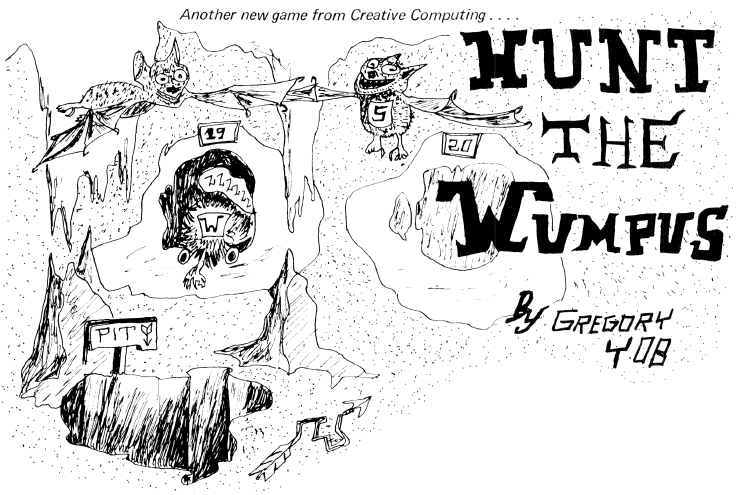
\includegraphics[width=0.7\textwidth]{images/wumpus.png}
  \caption{Hunt the Wumpus, an old turn based game where the human player can be completely substituded by an AI}
\end{figure}

However guaranteeing that opponents will be beaten is not the focus of commercial Turn-based Strategy games. For commercial games, if human players do not win, they quit the game. This can result in horrific future sales. Therefore, keeping players engage in the game is much more important.

\section{Decision making in turn based games}

Decision making is the ability of a character to decide what to do, is typically a small part of the effort needed to build great game AI.
Most games use very simple decision making systems: state machines and decision trees.
Rule-based systems are rarer, but important.
The character processes a set of information that it uses to generate an action that it wants to carry out. The input to the decision making system is the knowledge that a character possesses, and the output is an action request. The knowledge can be further broken down into external and internal knowledge. External knowledge is the information that a character knows about the game environment around it: the position of other characters, the layout of the level, whether a switch has been thrown, the direction that a noise is coming from, and so on. Internal knowledge is information about the character's internal state or thought processes: its health, its ultimate goals, what it was doing a couple of seconds ago, and so on.
\footnote{In our game external knowledge is composed by the position of the opponent plane, an estimation of his remaining life points and the world bounds, the internal knowledge is composed by own life points and own position}

Most common decision making systems today are decision trees, hieararchical state machines, scripting systems, minimax search, pathfinding (i.e A*). It's possible to arrange them in two \textit{macro-groups}: the non-search \textit{team} (decision trees, state machines...) and the search \textit{team} (minmax, planning...).
A \textbf{non-search} approach guarantees a predictable amount of computation 	(at cost of the amount of data stored), a \textbf{search} approach act in a different way and the only upper bound of the computation amount is relative to the search space
\footnote{Search based AI approach is usually \textbf{preferred in non realtime games} due to the computation resources in terms of power/time/memory needed} (which can be huge really often!)
